\chapter{Testing and Evaluation}

\label{chapter:evaluation}

In this chapter we present how the testing and evaluation of the proxy was
performed and present the results we obtained.  The goal is to measure any
possible improvements (or deterioration) of the performance of Web services
using the developed proxies. Then, based on these measurements, we give a
recommendation about which adaptations to make in different types of DIL
networks. Since the proxy was developed as a prototype for military usage, we
wanted to use test scenarios that resemble actual military and civilian usage.
For the purpose of testing, we therefore developed two sets of applications, one
W3C Web service and one RESTful Web service. These applications were then put to
test in networks with different characteristics. In addition, we also performed
some experiments where we researched how the size of a single request affected
the performance of CoAP.


We get started by discussing the test and evaluation tools used, before we
introduce the different test applications, test cases and the different types of
networks used for testing. Then we present the test results for each of the
three aspects of DIL, \textit{disconnected, intermittent} and \textit{limited.}
The aspects were tested separately. We started with the disconnected and
intermittent tests, where we investigated the behavior when connection was
lost. For the limited tests, we saw how different types of networks influenced
the performance of Web services. The base case was to test without any
intentional limitations to the network and without the actual usage of the
proxy. Then, we introduced usage of the proxy and evaluated it in different types
of limited networks.

Furthermore, we performed the tests with two different setups. First with an
emulator that emulates DIL networks, then we supplemented with testing over
actual military communication equipment. The usage of actual military equipment
allowed us to validate the results from the emulation testing.

\section{Types of DIL Networks}

Military communication can occur over a wide range of different technologies and
environments. These include \gls{satcom}, \gls{los},
\gls{cnr} and WiFi. WiFi is divided into two types to illustrate both
with good connection and one with less. Some communication technology, such as
satellite communication, is characterized by long communication delay while
others may be by their low data rate. An overview of selected military
communication technologies can be seen in \cref{figure-networks-overview}.

\begin{figure}[h]
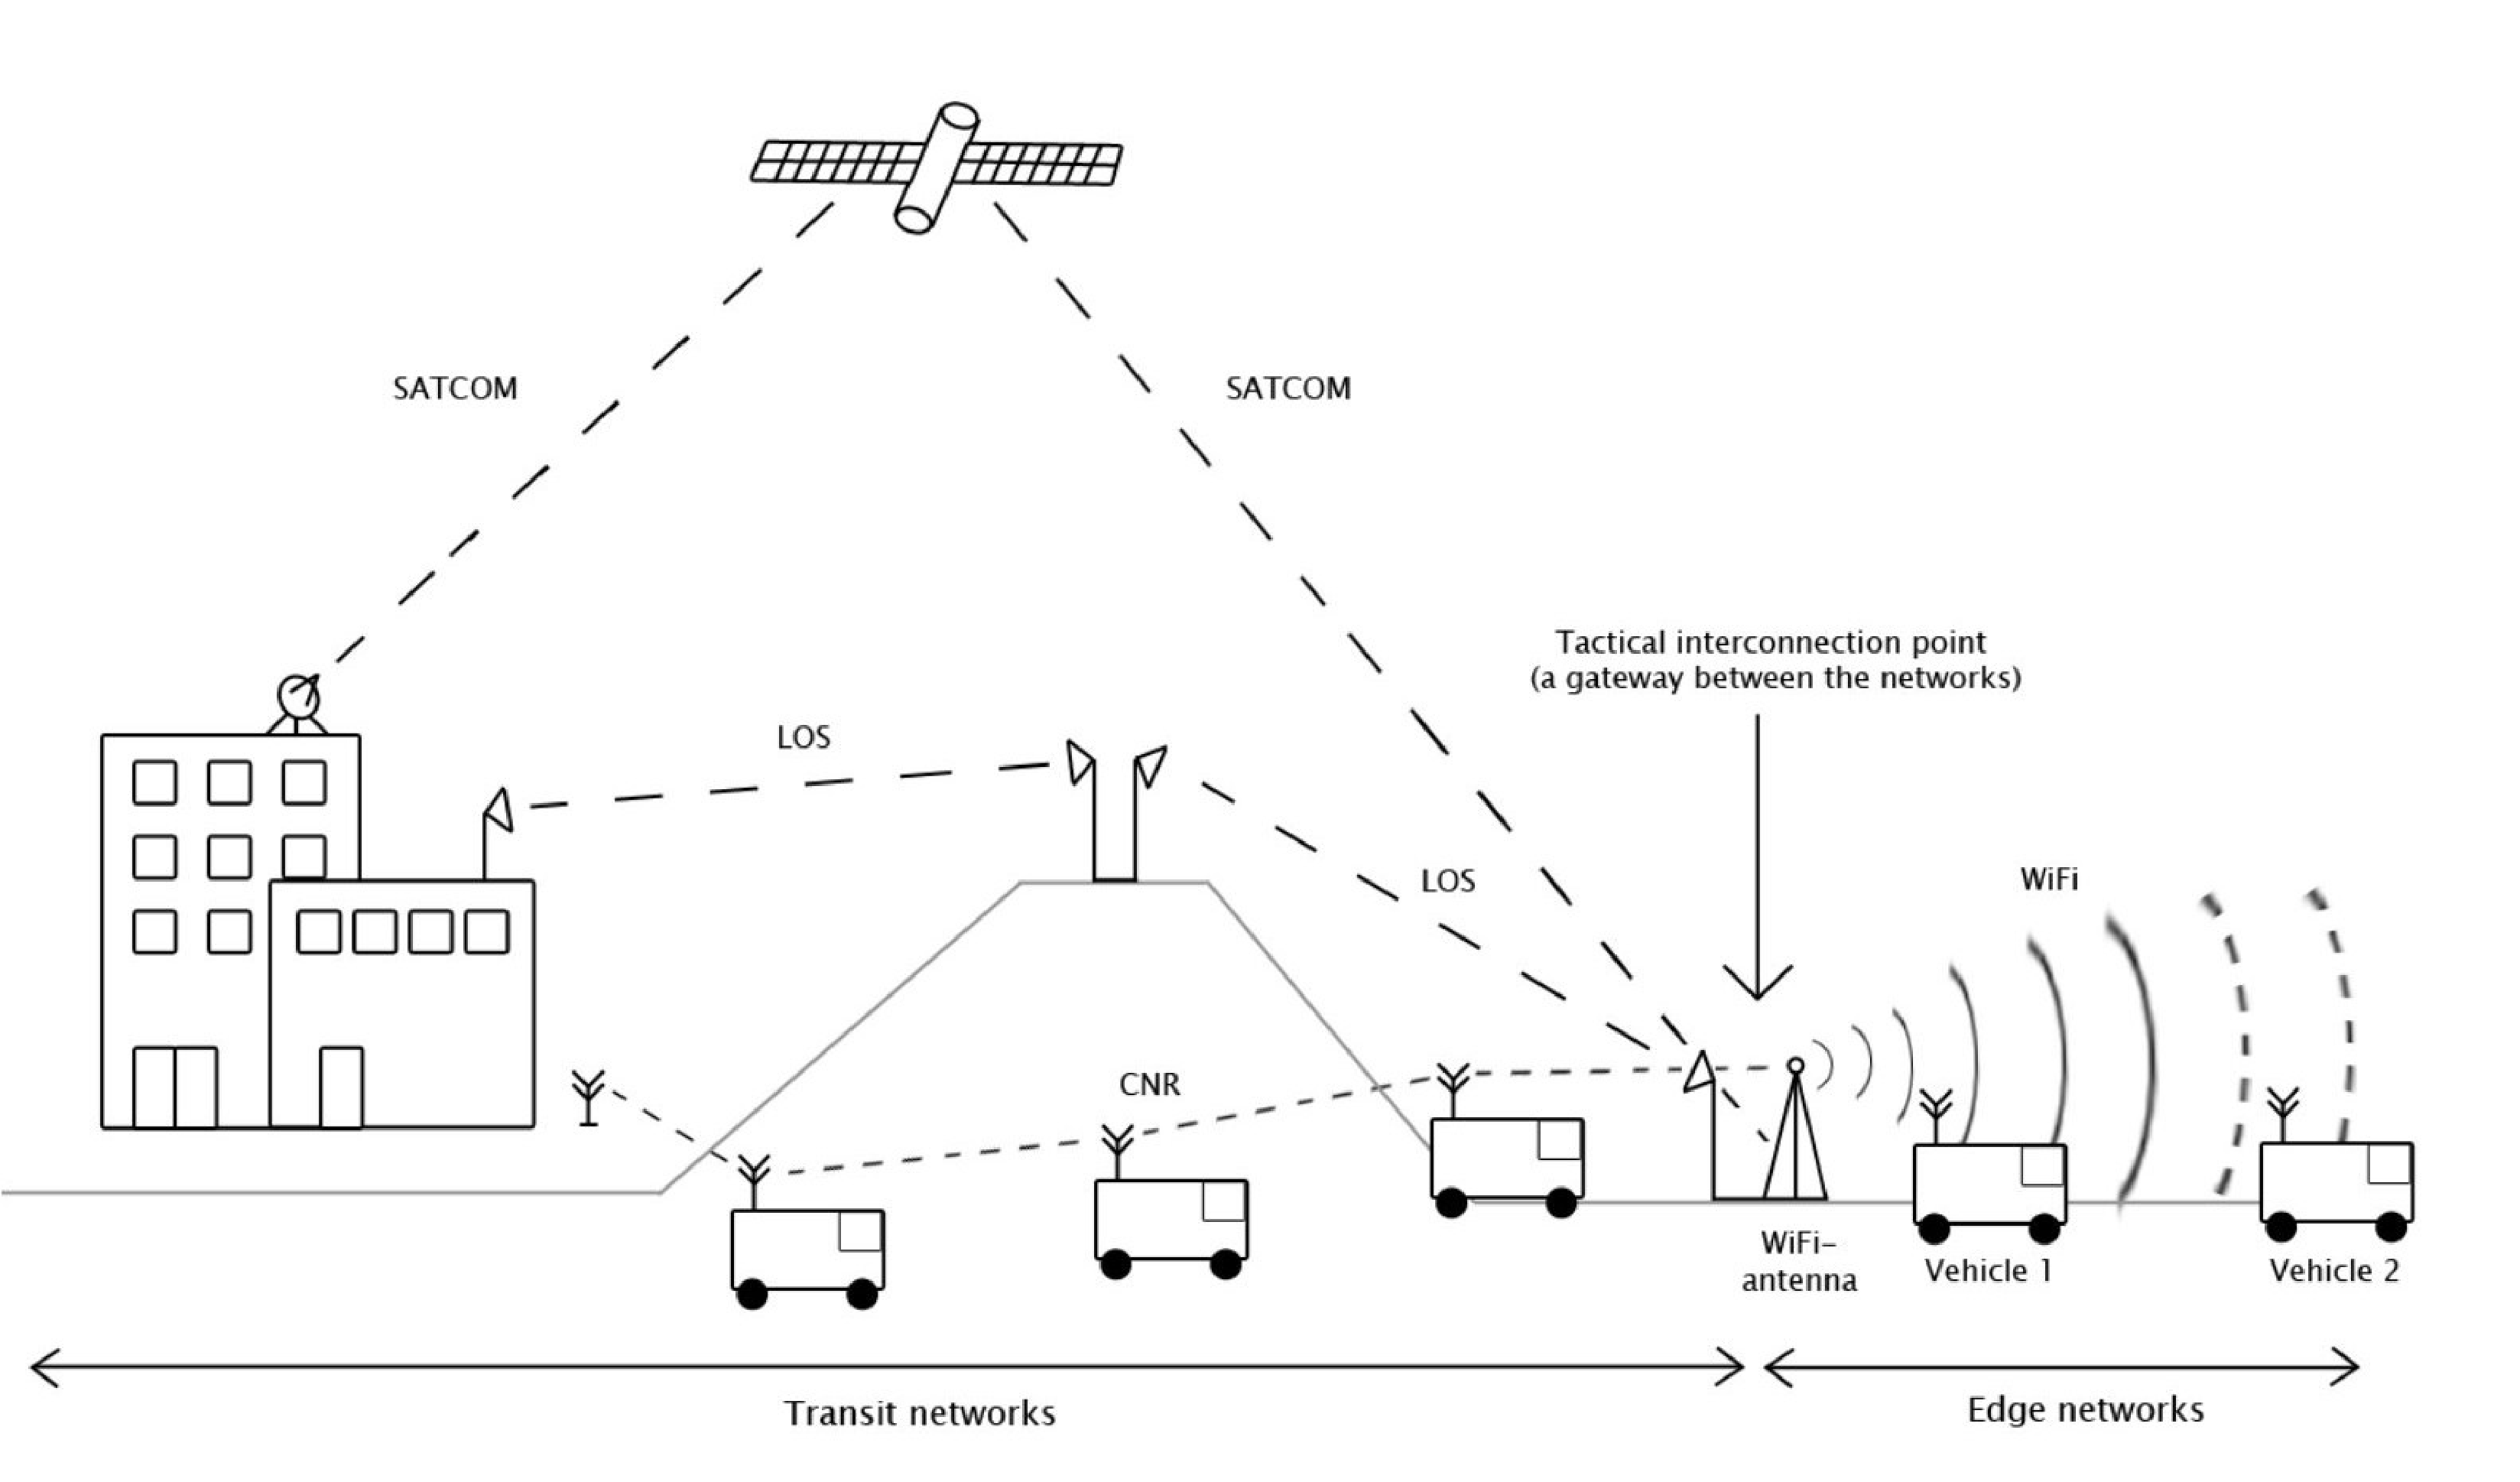
\includegraphics[scale=0.25]{images/networks_overview.pdf}
\caption{Overview of tested networks (from \cite{krog-pisa})}
\label{figure-networks-overview}
\end{figure}

An infinite number of possible network combinations exist, so we have chosen to
focus on five different network types identified by the task group IST-118 for
DIL-testing. The networks were identified because they represent typical
networks typically found in military communication. We also investigated
\gls{lte}, commonly known as 4G, a network technology which has become in
widespread use in the latest years. The reason for including LTE in addition to
the ones from IST-118, is that the Norwegian Defense is looking into the
possibility of using LTE. This makes it interesting for us to investigate the
performance under this type of network as well. However, we eventually found out
that LTE has gotten so fast and reliable, that it is not really relevant from a
DIL perspective. We therefore instead looked into \gls{edge}, which is used as a
fall back in geographical areas where \gls{lte} and 3G is not available. Of the
networks we evaluate for, is EDGE the only one with asymmetrical down- and
upload speed: 50 kbps up and 200 kbps down.

The different networks and their properties are summarized in
\cref{table-network-types}.

\begin{table}[h]
\begin{tabular}{| l | l | l | l | l |}
\hline
  \textbf{Network} & \textbf{Data Rate} & \textbf{Delay} & \textbf{PER} \\ \hline
  \gls{satcom} & 250 kbps & 550 ms & 0 \% \\ \hline
  \gls{los} & 2 mbps & 5 ms & 0 \% \\ \hline
  WiFi 1 & 2 mbps & 100 ms & 1 \% \\ \hline
  WiFi 2 & 2 mbps & 100 ms & 20 \% \\ \hline
  \gls{cnr} & 9.6 kbps & 100 ms & 1 \% \\ \hline
  \gls{edge} & 50 kbps up/200 kbps down & 200 ms & 0 \% \\ \hline
\end{tabular}
\caption{Different network types}
\label{table-network-types}
\end{table}


\section{Testing and Evaluation Tools}

In order to evaluate how our solution impacts the performance of Web services in
DIL environments, we needed some way of simulating such environments. Obviously,
we would have got the most realistic test environment by testing "out in the
field" ourselves. However, this would require of a considerable amount of effort
and it would be difficult to reproduce the exact same environment and test
results. We therefore choose to emulate DIL networks instead. For testing we used
two approaches, the first one connecting two machines through a third machine.
The third machine used a component in the Linux kernel to control the flow
of the network traffic flowing through it, allowing us to simulate DIL networks.
The second approach involved using actual military equipment in a laboratory at
FFI. The benefit of using actual equipment is that we got as realistic tests as
possible.


\subsection{Linux Network Traffic Control}

The Linux kernel offers a rich set of tools for managing and manipulating the
transmission of packets. \textbf{tc} (traffic control) is a Linux program to
configure and control the Linux kernels network scheduler. The central concept
in traffic controlling is the concept of queues, which collects entering packets
and dequeues them as fast as the network hardware can accept them. The
\gls{netem} is an enhancement of the traffic control facilities that allows us
to control delay, packet loss and other characteristics to packets outgoing from
a selected network interface \cite{man-netem}. These tools allow us to emulate
different network characteristics, for which we use to emulate the networks
listed in \cref{table-network-types}. For reference,
\cref{appendix-netem-scripts} of the appendix lists the NetEm scripts used.

How we configure \gls{netem} and the Linux traffic control tools to do this is
outlined in the following paragraphs.


\subsubsection{Emulating Network Delays}

NetEm can emulate delays on packets on a specific link. In
\cref{listing-netem-delay} we show an example configuration where a fixed delay
on 100 ms to all packets going out of local Ethernet connection.

\begin{lstlisting}[frame=single, caption="Emulating delay", label=listing-netem-delay]
  tc qdisc add dev eth0 parent 1:1 handle 10: \
    netem delay 100ms
\end{lstlisting}

\subsubsection{Emulating the Data Rate}

To emulate different data rates we use a part of the Linux traffic control tool
called \gls{tbf}. TBF can be used to shape network traffic and ensures that the
configured rate is not exceeded. It shapes traffic based on the concept of
\textit{tokens} and \textit{buckets}. Tokens are generated at a desired data
rate and are collected into buckets, which has a maximum number of tokens they
can store. When TBF receives a packet, it checks if it has sufficient number of
tokens in order to send the packet. If not, it is deferred, thus causing an
artificial delay for the packet.

\Cref{listing-netem-data-rate} shows an example configuration where we configure
the maximum data rate of 50 kilobits per second. The burst value is the size of
the bucket in bytes and describes the maximum amount of bytes that tokens can be
available for instantaneously. Limit is the number of bytes that can be queued
waiting for tokens to be available.

\begin{lstlisting}[frame=single, caption="Emulating data rate", label=listing-netem-data-rate]
  tc qdisc add dev eth0 handle 1: \
    root tbf rate 50kbit burst 15000 limit 15000
\end{lstlisting}

\subsubsection{Emulating the Corruption Rate}

The corrupt rate allows us to insert random data into a chosen percent of
packets. In \cref{listing-netem-error-rate} we show how the corruption rate can
be set to 20 percent.

\begin{lstlisting}[frame=single, caption="Emulating corruption rate", label=listing-netem-error-rate]
  tc qdisc add dev eth0 parent 1:1 handle 10: \
    netem delay 100ms corrupt 20%
\end{lstlisting}


\subsection{iPerf 3}

iPerf 3 is a tool for measurement of maximum achievable date rate on a
network \cite{iperf3-homepage}. Since we in this thesis are \textit{emulating}
different DIL networks, it is critical that the emulation is as correct and
realistic as possible. Misconfiguration or wrongful emulation could in the worst
case lead to us drawing invalid conclusions. To confirm and validate our network
emulations, we therefore used iPerf 3 alongside the Linux tool \textit{ping} to
confirm that the \gls{netem} scripts worked as expected. The measurements were
performed between the machine hosting the client and the machine hosting the Web
service. They were performed before starting the test cases so that the network
traffic it generated would not interfere.

Cite at iPerf 3 har blitt evaluert til beste måleverktøy. Vurdere å ta med graf som viser de ulike målingene med iPerf.

\subsection{Wireshark}

Wireshark is a packet analyzer and allows for performing network
analysis \cite{wireshark-homepage}. As an example, this tool allows a user to
see all IP packets sent from a machine over the Ethernet interface.

When performing the testing, we used Wireshark to monitor the network traffic on
the machine hosting the client and the local proxy. This allowed us to
investigate the behavior of the evaluated protocols in the different types of
networks. In particular we used it to see how many packets that were sent, as
well as total number of bytes that were sent over the network. Moreover, we used
it to see how long a HTTP request from a client was processed by the proxy
before it was forwarded. This enabled us to calculate how much processing time the
proxy used on a request, thus saying something about the CPU overhead of the proxy.

\section{Test Setup}
\label{testing-environment}

The majority of testing was performed at the FFI-lab at Kjeller. All the test
applications consisted of one client and one Web service, where the client would
request the service for some sort of data. The client where hosted on one
computer and the service on another computer. The majority of testing was
done using NetEm to emulate DIL networks, and some testing was done using actual
military radios. The machines used for testing are listed in
\cref{table-machines}.

\begin{table}[h]
\begin{tabularx}{\textwidth}{| l | X | X | X |}
\hline
  \textbf{Machine} & \textbf{Client} & \textbf{Application server} & \textbf{Router}\\ \hline
  Model & Asus UX 31A Notebook & HP EliteBook 6930p & HP Compaq Elite 8000 \\ \hline
  OS & Debian 8.2 & Ubuntu 14.04 & Ubuntu 14.04\\ \hline
  Kernel & 3.16.0-4-amd64 & 3.13.0-79-generic & 3.19.0-25-generic\\ \hline
  CPU & Intel i7 @ 1.90GHz & Intel Duo T95550 & Intel Quad Q9500 @ 2.83GHz \\ \hline
  Cores & 4 & 2 & 4\\ \hline
  Memory & 4 GB & 4 GB & 12 GB\\ \hline
  Network hardware & ASIX AX88772 USB 2.0 & 82567LM Gigabit & 82567LM-3 Gigabit\\ \hline
  Network interface capacity & 100 Mbit/s & 1 Gbit/s & 1 Gbit/s \\ \hline
\end{tabularx}
\caption{Machines involved in the testing}
\label{table-machines}
\end{table}

\subsection{NetEm Setup}

In this setup, the client and Web service machines were connected to each other
through a third computer, acting as a router. This router machine had two
network cards and networked together the other machines by Ethernet cables. The
setup can been seen in \cref{figure-testing-environment}. In order for the
router machine to forward IP packets back and forth between the client and
server, IP forwarding was enabled on the kernel.

\begin{figure}[h]
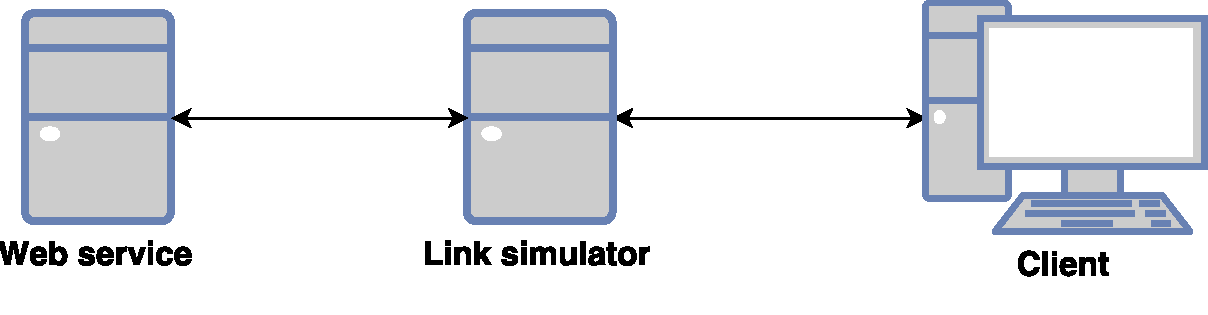
\includegraphics[scale=0.73]{images/testing_environment.pdf}
\caption{Test setup network}
\label{figure-testing-environment}
\end{figure}

The server and client are assigned an IP address in two different subnets.
This is done by the Linux network interface administration program
\textit{ifconfig}. In \cref{listing-ifconfig-client} the client machine is
assigned the IP address 192.168.11.44.

\begin{lstlisting}[frame=single, caption="Configuring a network interface of the router", label=listing-ifconfig-client]
ifconfig eth0 192.168.2.1 up
\end{lstlisting}

After setting up the IP addresses we need to configure the routing so that the
kernel knows where to route the network traffic. In this case we want all
traffic to go through the routing machine. In \cref{listing-routing} we
configure all IP traffic bound for the subnet 192.168.10 to be routed through
the router machine with IP 192.168.11.1.

\begin{lstlisting}[frame=single, caption="Configuring routing rules for the client", label=listing-routing]
ip route add unicast 192.168.10.0/24 via 192.168.11.1
\end{lstlisting}

\subsubsection{Emulating Different Types of Networks}

Since all network traffic passes through the routing machine, we can control the
flow of IP packets here. As previously discussed, we use NetEm.  For each
network configuration, a bash script is run. This script configures the network
interfaces in order to get the correct network behavior. Both interfaces are
configured so the network is symmetrical in both directions, with the exception
of EDGE which has asymmetrical data rates.

\subsection{Tactical Broadband Setup}

The majority of testing was performed over emulated networks. In addition, to
validate these results we performed tests on military communication equipment.
We used WM600 radios developed by \gls{kda}, intended for users "on-the-move".
WM600 can be used as IP radios through the Ethernet interface and support data
rates up to 2500 kbit/s \cite{kongsberg-wm600}. A picture of the radio can be
seen in \cref{figure-kdawm600}.


\begin{figure}[h]
\centering
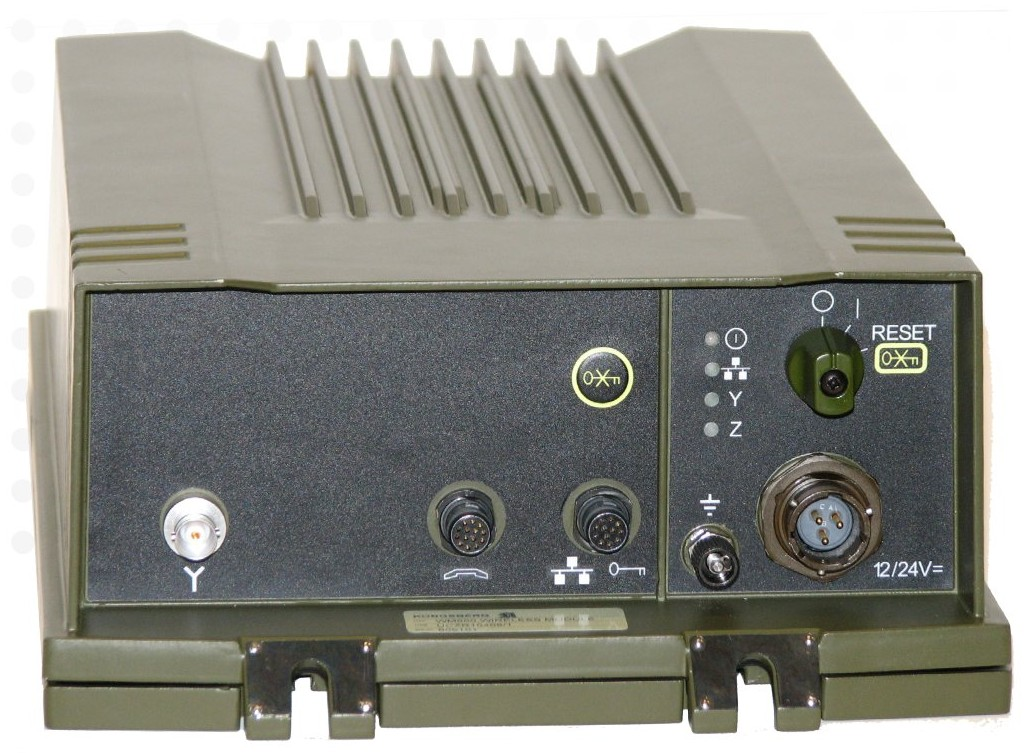
\includegraphics[scale=0.2]{images/kda_wm600.jpg}
\caption{The KDA WM600 radio (from \cite{kongsberg-wm600})}
\label{figure-kdawm600}
\end{figure}

We performed the testing at a communication laboratory at \gls{ffi} with the
setup illustrated in \cref{figure-radio-testing-environment}. It is a
point-to-point setup with two radios, without any multi hop functionality. The
radios have capacity to work as a multi hop \gls{manet}, but this was not tested
in this thesis.


\begin{figure}[h]
\centering
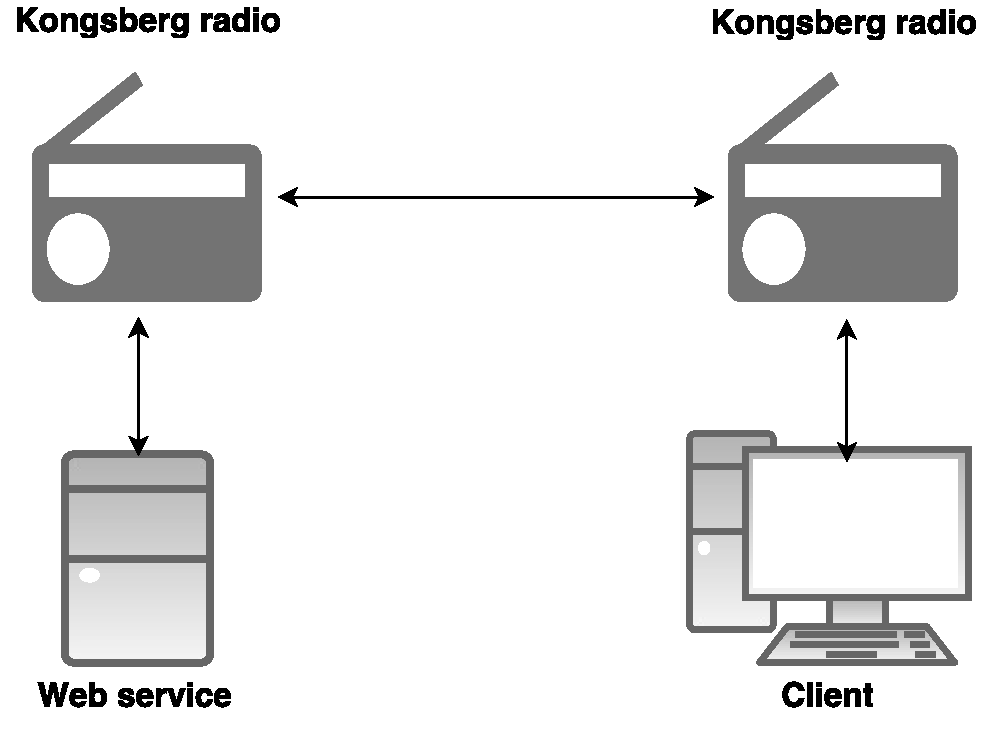
\includegraphics[scale=0.6]{images/radio_testing_environment.pdf}
\caption{Testing environment}
\label{figure-radio-testing-environment}
\end{figure}

\subsection{Proxy Setup}

For all test cases, the proxies ran on the same machine as their intended users.
The client and its proxy ran on one machine, while the Web service and its proxy
ran on another machine. Running on the Web service machine was also the message
broker, used by test cases involving AMQP.

\section{Test Execution}

 Each test scenario was performed with both a W3C Web service application and a
 RESTful Web service application. Each service is deployed in Glassfish 4, while
 the client is executed either from the command line or directly from the
 Netbeans IDE. Data being sent between the client and server is by default sent
 uncompressed.

During testing we discovered that especially \gls{coap} was very sensitive to
the size of the messages being sent. We therefore also conducted some
experiments by running tests where we investigated how it behaved with messages
of different sizes.

\subsection{NFFI W3C Web Service}

For the purpose of testing W3C Web service applications we created a mock system
which allows a client to request a service to report positions of friendly
forces. The position report uses the \gls{nffi} format, which has an associated
XML schema with it. One test run is illustrated in \cref{figure-nffi-flow} and
consists of the client making a HTTP POST request to the Web service. Associated
with the request is an XML payload which tells the Web service which operation
to invoke. In our case, the service then returns an XML message containing a
large number of positions in the NFFI format.

\begin{figure}[h]
\centering
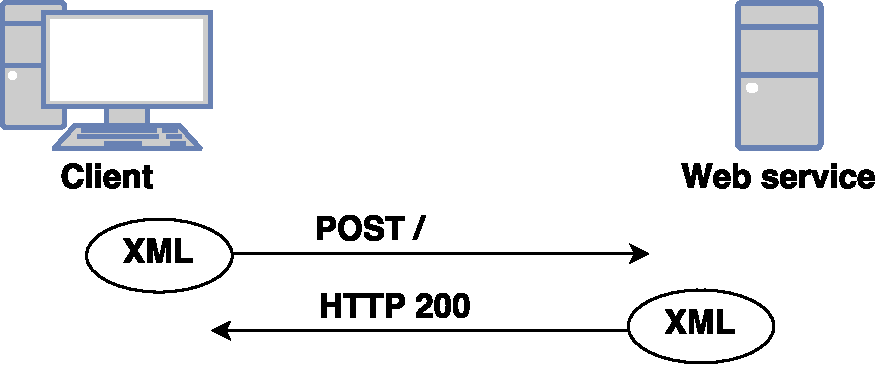
\includegraphics[scale=0.6]{images/nffi_flow.pdf}
\caption{NFFI Web service}
\label{figure-nffi-flow}
\end{figure}

\begin{table}[h]
\begin{tabular}{|l|l|l|l|}
\hline
\textbf{Request URI} & \textbf{HTTP Method} & \textbf{Bytes sent} & \textbf{Bytes received} \\ \hline
?wsdl                & GET                  & 192                 & 3527           \\ \hline
?wsdl=1              & GET                  & 194                 & 4331           \\ \hline
/                    & POST                 & 829                 & 40631          \\ \hline
\textbf{Total:}       & \textbf{3}                     & \textbf{1215}                & \textbf{48489}          \\ \hline
\end{tabular}
\caption{NFFI Web service HTTP requests}
\end{table}


\subsection{RESTful Car Service}

We originally wanted to use a service resembling a military scenario like the
NFFI service. However, no such applications were easily available for testing at
the time of writing the thesis. For the purpose of testing RESTful services, we
therefore chose to develop a small example service ourselves. The RESTful Car
service is a service keeping order of cars in a ``car system''. The service
exposes an \gls{api} which offers different operations to manage the car system.
Clients can invoke these operations by using HTTP requests and utilizing the
associated HTTP method to indicate what to do with a resource. Since RESTful
services are payload agnostic, we chose \gls{json} to represent the data being
sent between the server and the client. An example of usage of the Car system is
illustrated in \cref{figure-rest-flow}.

\begin{figure}[h]
\centering
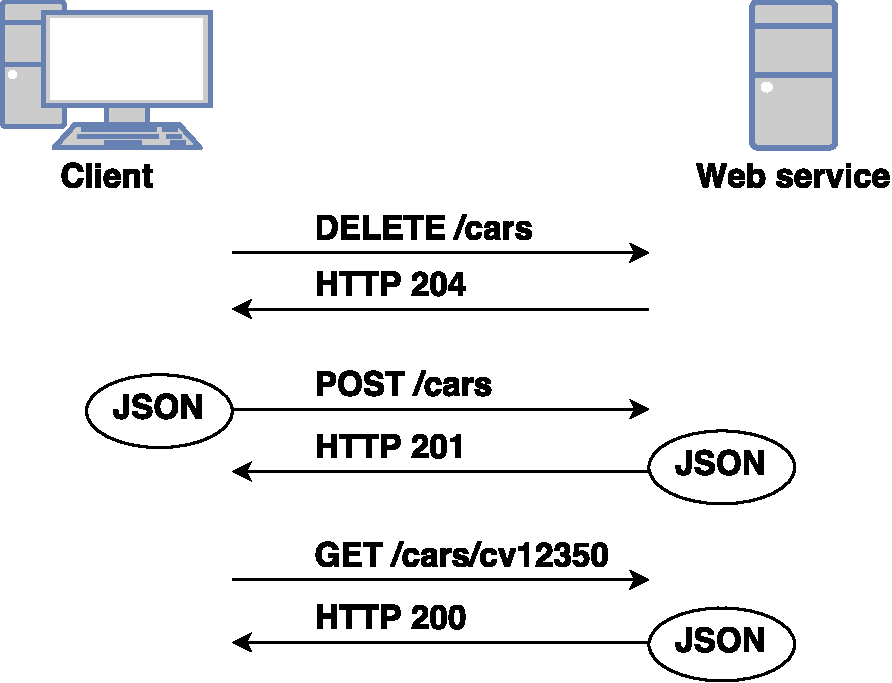
\includegraphics[scale=0.6]{images/rest_flow.pdf}
\caption{RESTful car service}
\label{figure-rest-flow}
\end{figure}

 Each test run of the Car system consist of a client sequentially invoking the
 server with different API requests, listed in \cref{table:car-requests}. The
 most common HTTP-methods GET, PUT, POST, and DELETE are all part of the
 tests.



\begin{table}[h]
\begin{tabular}{|l|l|l|l|}
\hline
\textbf{Request URI} & \textbf{HTTP Method} & \textbf{Bytes sent} & \textbf{Bytes received} \\ \hline
/cars                   & DELETE                  & 233                 & 243           \\ \hline
/cars                   & POST                  & 293                 & 353           \\ \hline
/cars                    & POST                 & 298                 & 358           \\ \hline
/cars                    & POST                 & 294                 & 354           \\ \hline
/cars                    & POST                 & 299                 & 359           \\ \hline
/cars                    & POST                 & 296                 & 356           \\ \hline
/cars                    & GET                 & 198                 & 538           \\ \hline
/cars/{id}                    & GET                 & 209                 & 348           \\ \hline
/cars/{id}                    & PUT                 & 309                 & 243           \\ \hline
/cars/{id}                   & GET                 & 209                 & 354           \\ \hline
/cars/{id}                   & DELETE                 & 244                 & 243           \\ \hline
/cars/                   & GET                 & 198                 & 495           \\ \hline
\textbf{Total:}       & \textbf{12}               & \textbf{3080}                & \textbf{4244}          \\ \hline
\end{tabular}
\caption{RESTful Car Service HTTP requests}
\label{table:car-requests}
\end{table}


\subsection{CoAP Experiments}

During the test execution of the NFFI and Car System service, we discovered that
CoAP was very sensitive to size of the message it was supposed to send. In
addition to the two test applications, to learn more we also experimented
by sending messages of different sizes with CoAP.

To do this, we used the simple http-server\cite{http-server-homepage},
which runs on the node runtime. The HTTP-server was configured to serve
 three files of different sizes, 1, 2 500 bytes and 100 000 bytes.
 The values were chosen to trigger fragmentation at different network layers.
 Ethernet has a \gls{mtu} on around 1 500 bytes and IP on 65 535 bytes.
 Furthermore, we created a basic Java client to request these files.

\subsection{Test Execution}

The tests was performed with the following parameters:

\begin{itemize}
	\item GZIP compression on/off.
	\item Without and with proxies.
    \item Transport protocol used.
\end{itemize}

Each test execution was initiated from a Java client running on the "client"
machine. We then measured how long it took to complete all requests, thus
allowing us to measure the Route Trip Time (RTT). All tests were performed
multiple times in order to calculate the mean, standard deviation and variance.
The results used to create the graphs presented in the next sections, are
included in the appendix, \cref{appendix-results}. For all networks, we also
tested without using the proxy. In those cases, requests were sent uncompressed
from the client to the Web service.


\subsection{Test Applications Summary}

A test run for the NFFI service and the RESTful Car service consist of
sequentially sending HTTP requests to their respective Web service. However,
they have some fundamental differences:

\begin{itemize}

     \item The Car system test involves running 12 HTTP requests, while the NFFI
     request only invokes three.

    \item The payload of each request response is generally is much smaller for
    the Car system tests. Moreover, the response message of the third request of the NFFI
    service is significantly larger than any other request or response.

\end{itemize}

\section{Function Tests}

The first phase of the testing is performed without any actual intended
limitations to the network. The objective of the function tests is to validate
that the proxy fulfill the functional requirements we set:

\begin{itemize}
    \item Receive and forward HTTP requests.
    \item Retain HTTP request and response headers.
    \item Support GZIP compression of payload.
    \item Support usage of different transport protocols between the proxies.
\end{itemize}

 In addition, the results from the function tests can be used to benchmark
 against other tests. The functional testing is divided into two phases, one
 without the usage of proxy and one with. Doing this allow us to investigate any
 potential overhead associated with the usage of the proxy. We used the NetEm
 setup with a third machine acting as a router, although without any intended
 limitations on the network. The tests are performed for both test applications
 and repeated multiple times to get the average \gls{rtt}.

\subsection{Results and Analysis}

Without using the proxy, \cref{figure:results-function-testsx} shows that for
both the NFFI and Car system test run, they both finish successfully within the
average time of 200 ms. When we introduce the proxies, all test cases still
complete successfully. The HTTP requests and responses are successfully
forwarded through the proxies, and the custom HTTP header set by the Car system is
retained. In the test cases without enabling compression, the usage of proxies
results in a longer RTT. This can be attributed to the overhead involved when
the proxy processes the requests and converts the message into the proxy message
format.

When compression is enabled and a HTTP proxy is used, we see a decrease in the RTT
for the NFFI test case. Inspecting the network traffic with Wireshark reveals
the probable cause for this. Compressing the relatively large XML documents sent
in NFFI test case yield a very high compression rates, while the compression rates
of the rather small JSON documents in the Car System test case are relatively
small. Furthermore, we observe that the transport protocol used by the proxies
has significant impact on the RTT and packets sent over the network.
\Cref{table:function-test-packets-nffi} and
\cref{table:function-test-packets-rest} list the IP packets sent over the
networks of one sample test run of the two test cases. In the following
paragraphs we discuss the behavior of the different protocols in use by the
proxies.

\subsubsection{HTTP Proxy}

For the NFFI test case with compression enabled, the HTTP proxy is marginally
faster than without the proxy. The reduction of data sent and received is
reflected by that the number of IP packets sent over the network are
significantly reduced, as seen in \cref{table:function-test-packets-nffi}.
Without compression, and for the Car system test case, the RTT is marginally
longer. The reason for this can be the overhead associated with the proxy. Using
Wireshark we analyzed one sample run of the Car system test and found the
following:

\begin{itemize}

	\item The first thing that happens when a test run is started, is that a TCP
	connection between the client application and the proxy is established. Then,
	the first HTTP DELETE request of the Car system test is sent from the
	application to the proxy. The request has no message body. Next, to be able to
	forward the request using HTTP, the proxy establishes a TCP connection with the
	other proxy.

	\item Then, a HTTP request is sent from the proxy to the other proxy. The
	DELETE request has now been converted to a POST request and the message
	body contains the proxy message. Since the request now has a message body,
	two HTTP headers has been appended: Content-Type and Content-Length. In
	addition, the HTTP-header breadcrumbID has been added. This is a header used
	by Camel. Including the proxy message, the size of the original HTTP request
	has now grown from 243 to 635 bytes.

	\item Next, the HTTP response is returned from the proxy. It consists of two
	reassembled TCP segments with the total size of 974  bytes. Comparing with the
	response from when not using a proxy, tell us a few things. Without the proxy,
	the response to the DELETE request is without a message body, while otherwise
	the custom proxy message is sent in the HTTP body. In addition, the response
	has additional HTTP headers than the original request. For this response, using
	the proxy had a message overhead of 756 bytes.

    \item In the consecutive HTTP requests the proxy did not need to establish a
    TCP connection since it was already open.

  \end{itemize}

As outlined above, using HTTP as the inter-proxy communication method caused an
overhead by including all of the HTTP request information in the proxy message.

\subsubsection{AMQP Proxy}

AMQP had the worst average RTT of the evaluated proxy protocols, especially for
the Car system test case. As seen in \cref{table:function-test-packets-nffi} and
\cref{table:function-test-packets-rest}, AMQP sends a lot more IP packets through
the network than HTTP. Since AMQP is broker based, communication occurs through a
message broker and not directly between the proxies. Using Wireshark, we dived
down into the details:

\begin{itemize}

	\item As with HTTP, a TCP connection between the test client and the
	proxy is first established. Then the proxy establish a TCP connection with the
	message broker.

	 \item Next, in order to forward the first HTTP request, the proxy initiates
	 an AMQP connection. This consists of numerous AMQP frames being sent between
	 the proxy and message broker. This includes exchanging the AMQP protocol
	 header and sending the AMQP frames Open, Begin, Attach and Flow.  First after
	 sending these frames, the first \textit{transfer} frame carrying the
	 message is sent.

     \item Finally, when a response is returned, both the AMQP and TCP connection
     are closed.

     \item When the next HTTP request is forwarded, these steps are repeated.

\end{itemize}

AMQP causes a significant overhead due to its complex connection procedures. For
every request that is forwarded through the proxy, a new AMQP and TCP connection
is established.

\subsubsection{CoAP Proxy}

Using CoAP as the inter-proxy communication protocol had roughly the same
average RTT as the HTTP proxy, with one exception. In the uncompressed NFFI test
case it had a longer RTT and sent a significant higher number of packets. We
believe this is due to some of the messages being so large, that a message has
to be split into multiple IP packets. This is called IP fragmentation. We
discuss CoAP and how it handles larger messages in section X.

For the test cases not involving large messages, CoAP sent significantly
\textit{fewer} IP packets than the other proxy protocols.

\begin{landscape}
    \begin{figure}
    \centering
    \begin{floatrow}
        \ffigbox[\FBwidth]
    {
    \subfloat[NFFI]{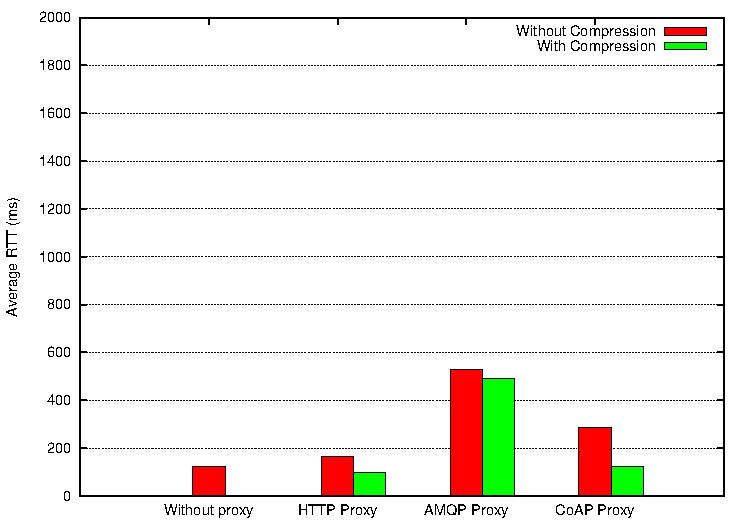
\includegraphics[width=0.5\textwidth]{../results/function_tests/nffi/output/result.pdf}}
    \subfloat[REST]{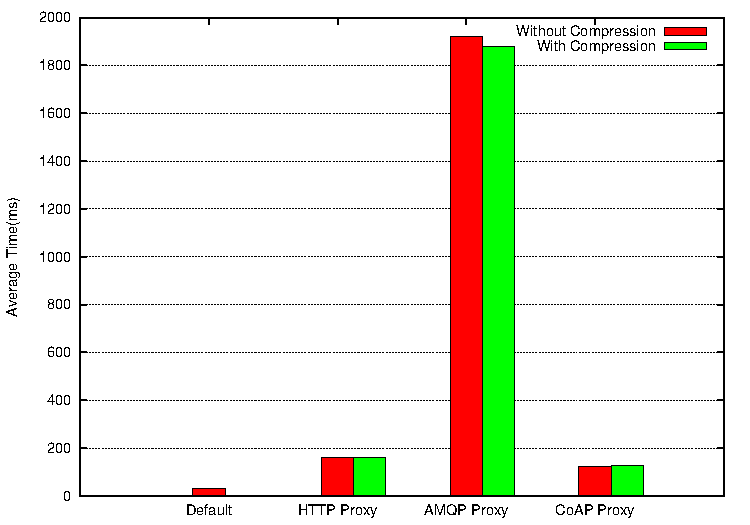
\includegraphics[width=0.5\textwidth]{../results/function_tests/rest/result.pdf}}
    }
    {
    \caption{Function tests - Average RTT Time for the client application.}
    \label{figure:results-function-testsx}
    }
    \end{floatrow}

    \end{figure}
\end{landscape}


\begin{table}[h]
\begin{tabular}{|l|l|l|}
\hline
\textbf{Test} & \textbf{Packets sent} & \textbf{Packets received} \\ \hline
Without Proxy                    &51         & 46        \\ \hline 
Proxy with HTTP                  &45         & 44        \\ \hline 
Proxy with HTTP \& GZIP          &13         & 13        \\ \hline 
Proxy with AMQP                  &73         & 94        \\ \hline 
Proxy with AMQP \& GZIP          &57         & 62        \\ \hline 
Proxy with CoAP                  &101        & 101       \\ \hline 
Proxy with CoAP \& GZIP          &11         & 11        \\ \hline 
\end{tabular}
\caption{NFFI Function test - IP Packets sent and received by the client application.}
\label{table:function-test-packets-nffi}
\end{table}

\begin{table}[h]
\begin{tabular}{|l|l|l|}
\hline
\textbf{Test} & \textbf{Packets sent} & \textbf{Packets received} \\ \hline
Without Proxy                    &25         & 21        \\ \hline 
Proxy with HTTP                  &28         & 26        \\ \hline 
Proxy with HTTP \& GZIP          &28         & 28        \\ \hline 
Proxy with AMQP                  &180        & 203       \\ \hline 
Proxy with AMQP \& GZIP          &190        & 207       \\ \hline 
Proxy with CoAP                  &12         & 12        \\ \hline 
Proxy with CoAP \& GZIP          &12         & 12        \\ \hline 
\end{tabular}
\caption{REST Function test - IP Packets sent and received by the client application.}
\label{table:function-test-packets-rest}
\end{table}


\section{DIL Tests - Intermittent and Disconnected}

\textit{Intermittent} and \textit{disconnected} refers to the network connection
being lost for some period of time, but then regained again. Disconnected
refers to loss of connection over a longer period, while intermittent is a
special case of disconnected and refers to shorter disruptions. In our testing
we focused on loss of connections for longer periods of time. The objective of
this testing is to evaluate how the proxy manages loss of connections over
periods of time. We define the success criteria for this test to be that the
client is able to eventually process his request after the connection is
reestablished. The clients HTTP request should not be interrupted in any way,
other than it taking longer time to process the request.

\subsection{Execution}

 The tests were performed on an unlimited network and were performed for
 both the NFFI and Car system service. They were executed by starting the test
 applications and then immediately removing the Ethernet cable between the
 client machine and the router machine. We then waited around 60 seconds,
 allowing requests to trigger timeouts and thus invoking the proxy’s redelivery
 mechanisms. Finally, we connected the cable again and observed if the test
 application were able to finish its requests successfully.


\subsection{Results and Analysis}

For both the REST and W3C Web service test scenarios the results were identical.
Without using proxies, the connection timed out and the applications were unable
to continue as shown in \cref{table:disconnected-nffi} and
\cref{table:disconnected-rest}. With proxies, the connection did not time out
and the protocols retransmission mechanisms were able to continue transmission
when connection was reestablished.


\begin{table}[h!]
\begin{tabular}{| l | l |}
\hline
  \textbf{Test} & \textbf{Result} \\ \hline
  Without proxy & Connection timeout \\ \hline
  Proxy with HTTP & Success \\ \hline
  Proxy with AMQP & Success \\ \hline
  Proxy with CoAP & Success \\ \hline
\end{tabular}
\caption{NFFI Web service results}
\label{table:disconnected-nffi}
\end{table}

\begin{table}[h!]
\begin{tabular}{| l | l |}
\hline
  \textbf{Test} & \textbf{Result} \\ \hline
  Without proxy & Connection timeout \\ \hline
  Proxy with HTTP & Success \\ \hline
  Proxy with AMQP & Success \\ \hline
  Proxy with CoAP & Success \\ \hline
\end{tabular}
\caption{RESTful Web service results}
\label{table:disconnected-rest}
\end{table}


\section{DIL Tests - Limited}

The third DIL characteristic, \textit{limited}, refers to different ways a
network can be limited. This includes high delays, packet loss and low
bandwidth. In this section we present the testing performed for the different
types of networks identified in \cref{table-network-types}.



\subsection{Satellite Communication}

In this test scenario we emulate \gls{satcom}. With satellite communication
all data is relayed through a communication satellite in orbit around
the earth. This type of communication is characterized by its low data rate
and high delay.

\subsubsection{Results and Analysis}

From the SATCOM testing results presented in \cref{figure:results-satcom},
\cref{table:satcom-test-packets-nffi} and \cref{table:satcom-test-packets-rest},
we observe the following:

\begin{itemize}

    \item Compression can be of less importance in networks where the high delay
    is the limiting factor.

    \item With one exception, AMQP has significantly higher RTT than the other
    protocols. For the Car system tests with many HTTP requests, we see that
    AMQP triggers the sending of many IP packets. In a sample test run the
    Wireshark capture revealed that AMQP sends twenty times the amount of IP packets
    compared to CoAP.

    \item CoAP struggles with the large messages of NFFI test case. In the Car
    system test case however, a Wireshark capture reveals that it sends few number of IP
    packets.

    \item The HTTP proxy with compression enabled has the overall best RTT. For
    the Car system test, CoAP has almost equal average RTT as the HTTP proxy.

\end{itemize}

\begin{landscape}
    \begin{figure}
    \centering
    \begin{floatrow}
        \ffigbox[\FBwidth]
    {
    \subfloat[NFFI]{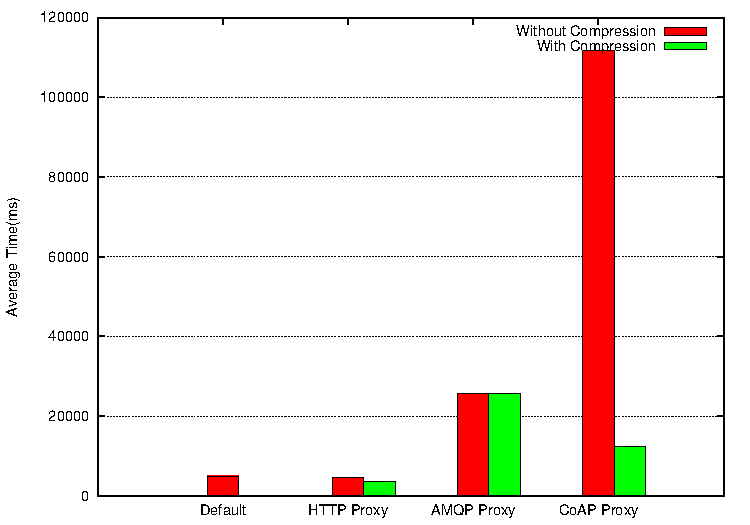
\includegraphics[width=0.5\textwidth]{../results/satellite/nffi/result.pdf}}
    \subfloat[REST]{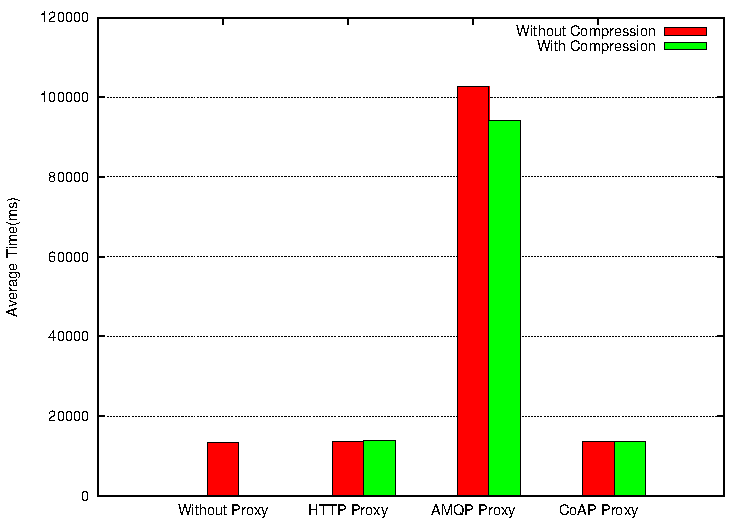
\includegraphics[width=0.5\textwidth]{../results/satellite/rest/result.pdf}}
    }{\caption{SATCOM tests - Average RTT Time for the client application.}
    \label{figure:results-satcom}
    }
    \end{floatrow}
    \end{figure}
\end{landscape}


\begin{table}[h]
\begin{tabular}{|l|l|l|}
\hline
\textbf{Test} & \textbf{Packets sent} & \textbf{Packets received} \\ \hline
Without Proxy                    &54         & 47        \\ \hline 
Proxy with HTTP                  &47         & 45        \\ \hline 
Proxy with HTTP \& GZIP          &16         & 14        \\ \hline 
Proxy with AMQP                  &88         & 102       \\ \hline 
Proxy with AMQP \& GZIP          &71         & 68        \\ \hline 
Proxy with CoAP                  &101        & 101       \\ \hline 
Proxy with CoAP \& GZIP          &11         & 11        \\ \hline 
\end{tabular}
\caption{NFFI SATCOM test - IP Packets sent and received by the client application.}
\label{table:satcom-test-packets-nffi}
\end{table}

\begin{table}[h]
\begin{tabular}{|l|l|l|}
\hline
\textbf{Test} & \textbf{Packets sent} & \textbf{Packets received} \\ \hline
Without Proxy                    &27         & 22        \\ \hline 
Proxy with HTTP                  &26         & 25        \\ \hline 
Proxy with HTTP \& GZIP          &30         & 28        \\ \hline 
Proxy with AMQP                  &244        & 238       \\ \hline 
Proxy with AMQP \& GZIP          &240        & 240       \\ \hline 
Proxy with CoAP                  &12         & 12        \\ \hline 
Proxy with CoAP \& GZIP          &12         & 12        \\ \hline 
\end{tabular}
\caption{REST SATCOM test - IP Packets sent and received by the client application.}
\label{table:satcom-test-packets-rest}
\end{table}




\subsection{Line-of-Sight}

In this test scenario we emulate \gls{los} networks, which are characterized by
being a radio-based type of network with no physical obstacles between the nodes
in the network. LOS has high data rate, low delay and zero error rate.

\subsubsection{Results and Analysis}

The average RTT of the LOS tests are shown in \cref{los:results-satcom}. IP
packets sent and received in a sample run of the NFFI and Car system test cases
are listed in \cref{table:los-test-packets-nffi} and
\cref{table:los-test-packets-rest}. The important findings are summarized here:

\begin{itemize}

    \item We observe the same trends regarding CoAP and AMQP as in the previous
    tested networks.

    \item Proxy with HTTP has the best RTT in the NFFI test case. In the Car
    system test, not using a proxy yields the best RTT.

    \item In the Car system test case, the CoAP proxy is marginally faster than a
    proxy with HTTP.

    \item The LOS type of network is a relatively unlimited network. The results
    has the same trends as the results from the function tests.

\end{itemize}



\begin{landscape}
    \begin{figure}
    \centering
    \begin{floatrow}
        \ffigbox[\FBwidth]
    {
    \subfloat[NFFI]{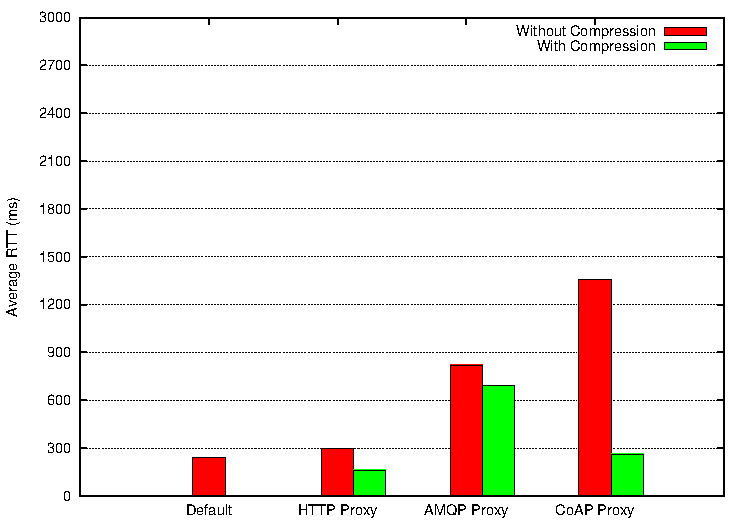
\includegraphics[width=0.5\textwidth]{../results/los/nffi/result.pdf}}
    \subfloat[REST]{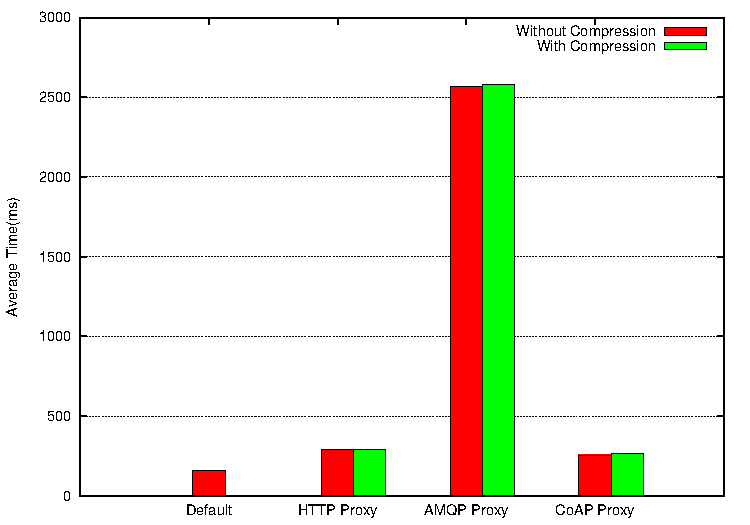
\includegraphics[width=0.5\textwidth]{../results/los/rest/result.pdf}}
    }{\caption{LOS tests - Average RTT Time for the client application.}
        \label{los:results-satcom}
    }
    \end{floatrow}
    \end{figure}
\end{landscape}

\begin{table}[h]
\begin{tabular}{|l|l|l|}
\hline
\textbf{Test} & \textbf{Packets sent} & \textbf{Packets received} \\ \hline
Without Proxy                    &46         & 43        \\ \hline 
Proxy with HTTP                  &43         & 44        \\ \hline 
Proxy with HTTP \& GZIP          &14         & 13        \\ \hline 
Proxy with AMQP                  &68         & 91        \\ \hline 
Proxy with AMQP \& GZIP          &54         & 59        \\ \hline 
Proxy with CoAP                  &101        & 101       \\ \hline 
Proxy with CoAP \& GZIP          &11         & 11        \\ \hline 
\end{tabular}
\caption{NFFI LOS test - IP Packets sent and received by the client application.}
\label{table:los-test-packets-nffi}
\end{table}

\begin{table}[h]
\begin{tabular}{|l|l|l|}
\hline
\textbf{Test} & \textbf{Packets sent} & \textbf{Packets received} \\ \hline
Without Proxy                    &25         & 21        \\ \hline 
Proxy with HTTP                  &28         & 26        \\ \hline 
Proxy with HTTP \& GZIP          &24         & 24        \\ \hline 
Proxy with AMQP                  &189        & 201       \\ \hline 
Proxy with AMQP \& GZIP          &187        & 201       \\ \hline 
Proxy with CoAP                  &12         & 12        \\ \hline 
Proxy with CoAP \& GZIP          &12         & 12        \\ \hline 
\end{tabular}
\caption{REST LOS test - IP Packets sent and received by the client application.}
\label{table:los-test-packets-rest}
\end{table}




\subsection{WiFi 1}

With this type of network we emulate communication over WiFi where the
conditions are relatively good. The data rate is high, the delay is moderate
and the packet error rate is 1 \%.

\subsubsection{Results and Analysis}

The results from the test in this type of network are presented in
\cref{figure:wifi1-results}, \cref{table:wifi1-test-packets-nffi} and
\cref{table:wifi1-test-packets-rest}. We see the following:

\begin{itemize}

    \item Again we observe the same trends from previous tests. AMQP has the
    longest RTT, while CoAP struggle with large messages.

    \item For the NFFI test, HTTP with compression enabled yields the lowest
    average RTT.

    \item For the Car system tests, running without using proxies have the
    lowest average RTT.

\end{itemize}


\begin{landscape}
    \begin{figure}
    \centering
    \begin{floatrow}
        \ffigbox[\FBwidth]
    {
    \subfloat[NFFI]{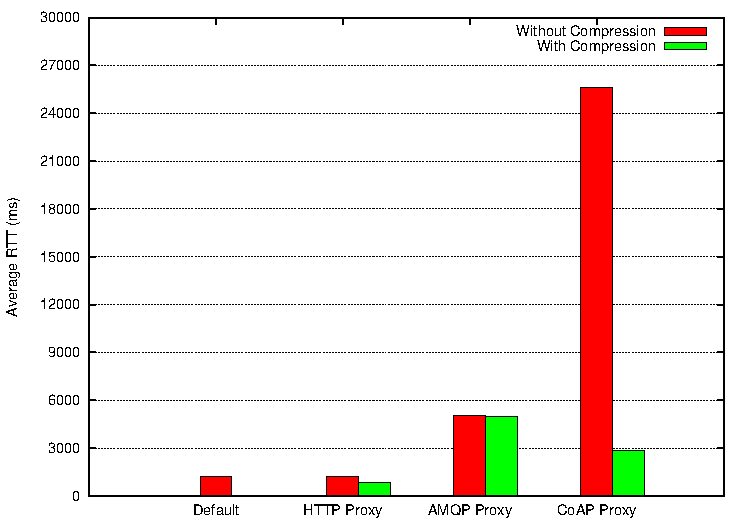
\includegraphics[width=0.5\textwidth]{../results/wifi1/nffi/result.pdf}}
    \subfloat[REST]{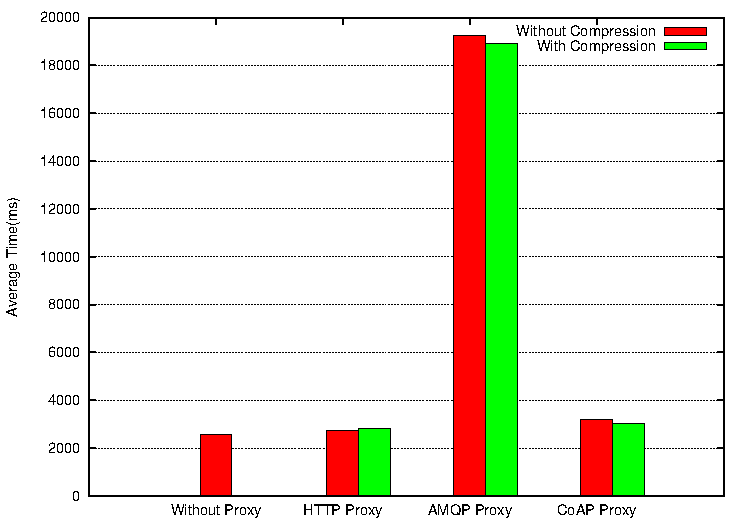
\includegraphics[width=0.5\textwidth]{../results/wifi1/rest/result.pdf}}
    }{\caption{WiFi 1 tests - Average RTT Time for the client application.}
\label{figure:wifi1-results}
    }
    \end{floatrow}
    \end{figure}
\end{landscape}

\begin{table}[h]
\begin{tabular}{|l|l|l|}
\hline
\textbf{Test} & \textbf{Packets sent} & \textbf{Packets received} \\ \hline
Without Proxy                    &50         & 45        \\ \hline 
Proxy with HTTP                  &45         & 45        \\ \hline 
Proxy with HTTP \& GZIP          &13         & 14        \\ \hline 
Proxy with AMQP                  &76         & 93        \\ \hline 
Proxy with AMQP \& GZIP          &60         & 60        \\ \hline 
Proxy with CoAP                  &104        & 104       \\ \hline 
Proxy with CoAP \& GZIP          &22         & 22        \\ \hline 
\end{tabular}
\caption{NFFI WiFi 1 test - IP Packets sent and received by the client application.}
\label{table:wifi1-test-packets-nffi}
\end{table}

\begin{table}[h]
\begin{tabular}{|l|l|l|}
\hline
\textbf{Test} & \textbf{Packets sent} & \textbf{Packets received} \\ \hline
Without Proxy                    &28         & 22        \\ \hline 
Proxy with HTTP                  &26         & 24        \\ \hline 
Proxy with HTTP \& GZIP          &30         & 27        \\ \hline 
Proxy with AMQP                  &192        & 211       \\ \hline 
Proxy with AMQP \& GZIP          &198        & 208       \\ \hline 
Proxy with CoAP                  &12         & 12        \\ \hline 
Proxy with CoAP \& GZIP          &12         & 12        \\ \hline 
\end{tabular}
\caption{REST WiFi 1 test - IP Packets sent and received by the client application.}
\label{table:wifi1-test-packets-rest}
\end{table}


\subsection{WiFi 2}

This type of network also emulate wireless communication, but instead in the
``outer'' areas of the wireless range. It has good data rate, moderate delay
and very high packet error rate (20 \%).


\subsubsection{Results and Analysis}

\Cref{figure:wifi2-results} shows the average response times of the WiFi 2 test
cases. \Cref{table:wifi2-test-packets-nffi} and
\cref{table:wifi2-test-packets-rest} list the packets sent and received from the
test applications in a sample test run. For the tests ran in an emulated WiFi 2
network, we see the following:

\begin{itemize}

    \item We observe a significantly longer average RTT for all test cases. The
    variance of the test results have increased compared to the other test
    networks. This can be attributed to the high probability of packet error,
    since some test runs may experience few errors, while other more.

    \item In the NFFI test case with CoAP without compression, the proxy was not
    able to forward the request. The reason for this is that the CoAP request
    between the proxies timed out. The retransmission mechanism of the proxy
    were invoked, but the consecutive attempts were unsuccessfully as well.
    Furthermore, we observe that even with compression did CoAP has a longer
    average RTT than the other protocols.

    \item We also see that for the NFFI test cases, compressing the messages
    yields a large performance increase with regards to the average RTT. This is
    probably due to since less IP packets need to be sent over the network, it
    is a less chance for packet errors.

    \item The HTTP proxy with compression enabled had the overall best average
    RTT.

\end{itemize}


\begin{landscape}
    \begin{figure}
    \centering
    \begin{floatrow}
        \ffigbox[\FBwidth]
    {
    \subfloat[NFFI]{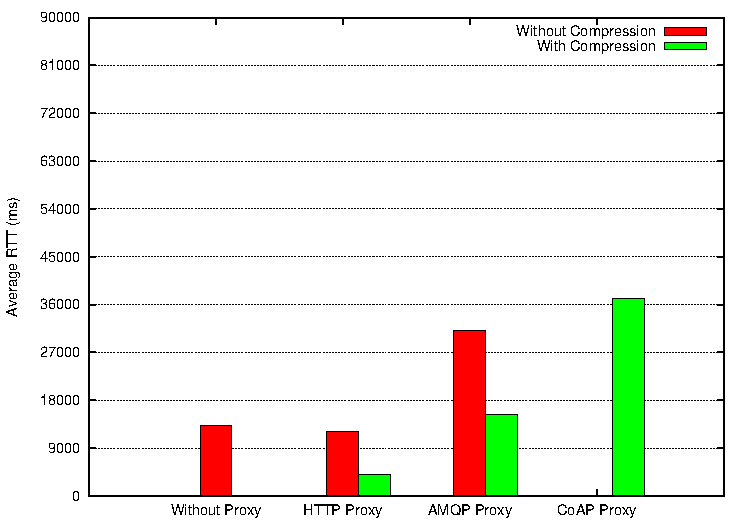
\includegraphics[width=0.5\textwidth]{../results/wifi2/nffi/result.pdf}}
    \subfloat[REST]{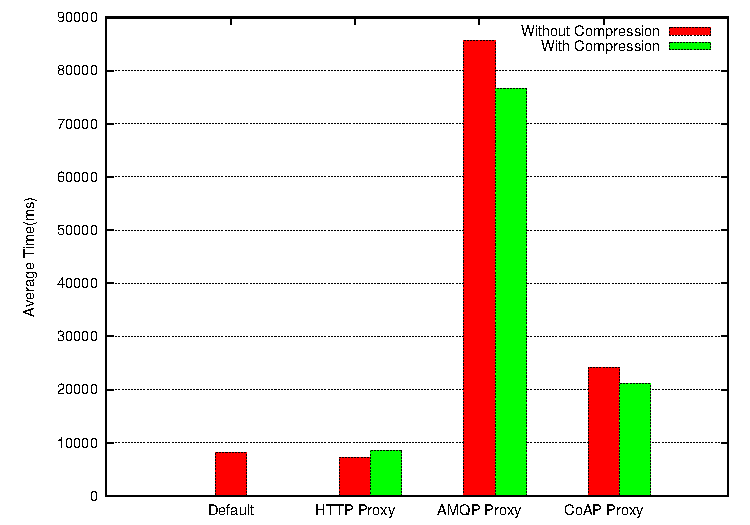
\includegraphics[width=0.5\textwidth]{../results/wifi2/rest/result.pdf}}
    }{\caption{WiFi 2 tests - Average RTT Time for the client application.}
\label{figure:wifi2-results}
    }
    \end{floatrow}
    \end{figure}
\end{landscape}

\begin{table}[h]
\begin{tabular}{|l|l|l|}
\hline
\textbf{Test} & \textbf{Packets sent} & \textbf{Packets received} \\ \hline
Without Proxy                    &51         & 54        \\ \hline 
Proxy with HTTP                  &45         & 52        \\ \hline 
Proxy with HTTP \& GZIP          &15         & 13        \\ \hline 
Proxy with AMQP                  &101        & 111       \\ \hline 
Proxy with AMQP \& GZIP          &76         & 71        \\ \hline 
Proxy with CoAP                  &0          & 0         \\ \hline 
Proxy with CoAP \& GZIP          &14         & 12        \\ \hline 
\end{tabular}
\caption{NFFI WiFi 2 test - IP Packets sent and received by the client application.}
\label{table:wifi2-test-packets-nffi}
\end{table}

\begin{table}[h]
\begin{tabular}{|l|l|l|}
\hline
\textbf{Test} & \textbf{Packets sent} & \textbf{Packets received} \\ \hline
Without Proxy                    &32         & 39        \\ \hline 
Proxy with HTTP                  &37         & 30        \\ \hline 
Proxy with HTTP \& GZIP          &31         & 28        \\ \hline 
Proxy with AMQP                  &332        & 317       \\ \hline 
Proxy with AMQP \& GZIP          &231        & 243       \\ \hline 
Proxy with CoAP                  &18         & 15        \\ \hline 
Proxy with CoAP \& GZIP          &24         & 17        \\ \hline 
\end{tabular}
\caption{REST WiFi 2 test - IP Packets sent and received by the client application.}
\label{table:wifi2-test-packets-rest}
\end{table}

\subsection{Combat Net Radio}

\gls{cnr} is characterized by very low data rate, moderate timeout and packet
error rate of around 1 \%.


\subsubsection{Results and Analysis}

Again we can observe the importance of compression in this type of networks.
CoAP has the best performance.

\begin{landscape}
    \begin{figure}
    \centering
    \begin{floatrow}
        \ffigbox[\FBwidth]
    {
    \subfloat[NFFI]{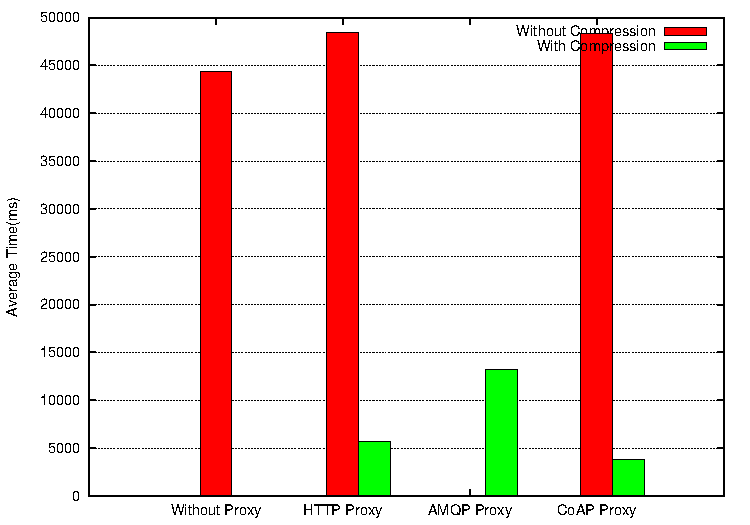
\includegraphics[width=0.5\textwidth]{../results/cnr/nffi/result.pdf}}
    \subfloat[REST]{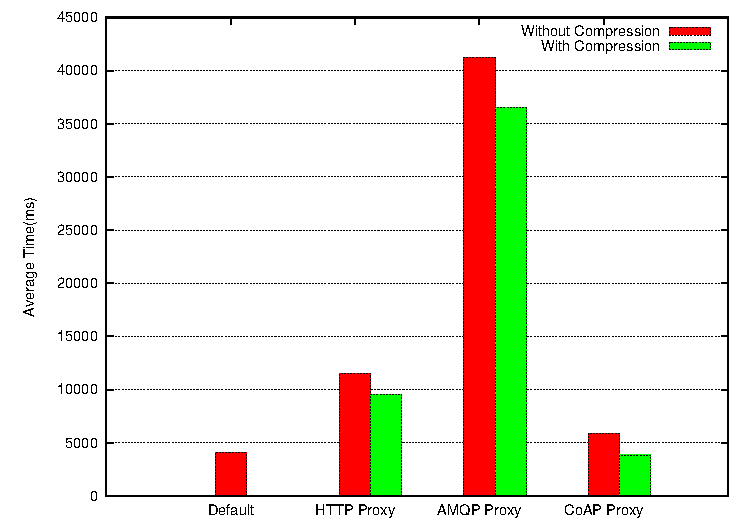
\includegraphics[width=0.5\textwidth]{../results/cnr/rest/result.pdf}}
    }{\caption{CNR tests - Average RTT Time for the client application.}}
    \end{floatrow}
    \end{figure}
\end{landscape}

\begin{table}[h]
\begin{tabular}{|l|l|l|}
\hline
\textbf{Test} & \textbf{Packets sent} & \textbf{Packets received} \\ \hline
Without Proxy                    &70         & 71        \\ \hline 
Proxy with HTTP                  &66         & 67        \\ \hline 
Proxy with HTTP \& GZIP          &14         & 13        \\ \hline 
Proxy with AMQP                  &0          & 0         \\ \hline 
Proxy with AMQP \& GZIP          &56         & 62        \\ \hline 
Proxy with CoAP                  &103        & 103       \\ \hline 
Proxy with CoAP \& GZIP          &11         & 11        \\ \hline 
\end{tabular}
\caption{NFFI CNR test - IP Packets sent and received by the client application.}
\end{table}

\begin{table}[h]
\begin{tabular}{|l|l|l|}
\hline
\textbf{Test} & \textbf{Packets sent} & \textbf{Packets received} \\ \hline
Without Proxy                    &25         & 21        \\ \hline 
Proxy with HTTP                  &28         & 27        \\ \hline 
Proxy with HTTP \& GZIP          &24         & 24        \\ \hline 
Proxy with AMQP                  &233        & 240       \\ \hline 
Proxy with AMQP \& GZIP          &220        & 225       \\ \hline 
Proxy with CoAP                  &14         & 13        \\ \hline 
Proxy with CoAP \& GZIP          &12         & 12        \\ \hline 
\end{tabular}
\caption{REST CNR test - IP Packets sent and received by the client application.}
\end{table}


\subsection{EDGE}

EDGE is characterized by a low upload data rate, and a moderately low download
rate. Furthermore, we emulate EDGE with a moderate delay and zero packet loss.

\begin{landscape}
    \begin{figure}
    \centering
    \begin{floatrow}
        \ffigbox[\FBwidth]
    {
    \subfloat[NFFI]{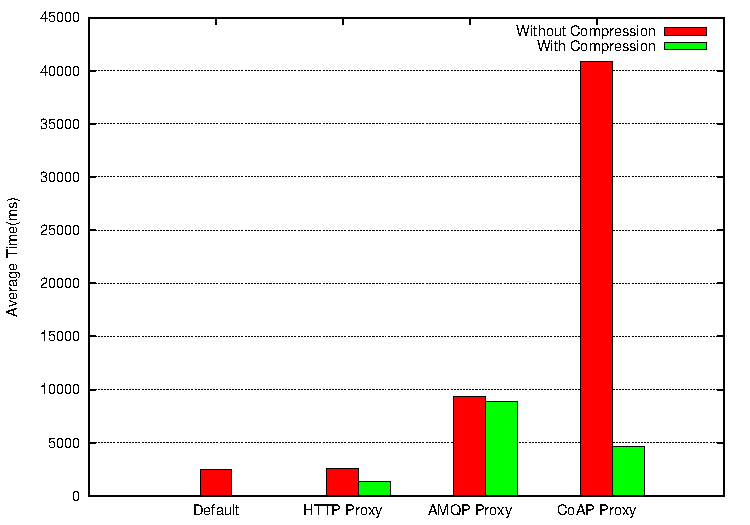
\includegraphics[width=0.5\textwidth]{../results/edge/nffi/result.pdf}}
    \subfloat[REST]{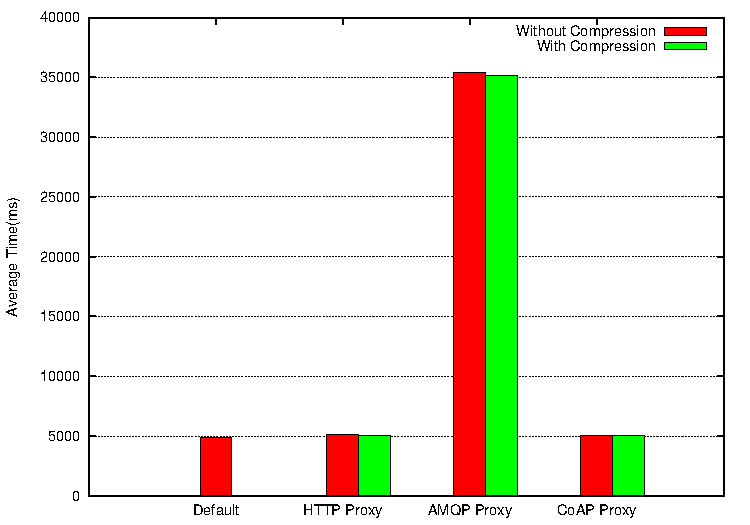
\includegraphics[width=0.5\textwidth]{../results/edge/rest/result.pdf}}
    }{\caption{EDGE tests - Average RTT Time for the client application.}}
    \end{floatrow}
    \end{figure}
\end{landscape}

\begin{table}[h]
\begin{tabular}{|l|l|l|}
\hline
\textbf{Test} & \textbf{Packets sent} & \textbf{Packets received} \\ \hline
Without Proxy                    &50         & 45        \\ \hline 
Proxy with HTTP                  &45         & 44        \\ \hline 
Proxy with HTTP \& GZIP          &14         & 13        \\ \hline 
Proxy with AMQP                  &78         & 95        \\ \hline 
Proxy with AMQP \& GZIP          &59         & 59        \\ \hline 
Proxy with CoAP                  &101        & 101       \\ \hline 
Proxy with CoAP \& GZIP          &11         & 11        \\ \hline 
\end{tabular}
\caption{NFFI CNR test - IP Packets sent and received by the client application.}
\end{table}

\begin{table}[h]
\begin{tabular}{|l|l|l|}
\hline
\textbf{Test} & \textbf{Packets sent} & \textbf{Packets received} \\ \hline
Without Proxy                    &27         & 23        \\ \hline 
Proxy with HTTP                  &28         & 27        \\ \hline 
Proxy with HTTP \& GZIP          &29         & 27        \\ \hline 
Proxy with AMQP                  &194        & 201       \\ \hline 
Proxy with AMQP \& GZIP          &201        & 212       \\ \hline 
Proxy with CoAP                  &12         & 12        \\ \hline 
Proxy with CoAP \& GZIP          &12         & 12        \\ \hline 
\end{tabular}
\caption{REST EDGE test - IP Packets sent and received by the client application.}
\end{table}

\subsection{Tactical Broadband}

In addition to the software emulated networks, we performed tests with KDA WM600
radios.


\subsubsection{Results and analysis}

For NFFI tests, compression yields a lot of increase in performance.

\begin{landscape}
    \begin{figure}
    \centering
    \begin{floatrow}
        \ffigbox[\FBwidth]
    {
    \subfloat[NFFI]{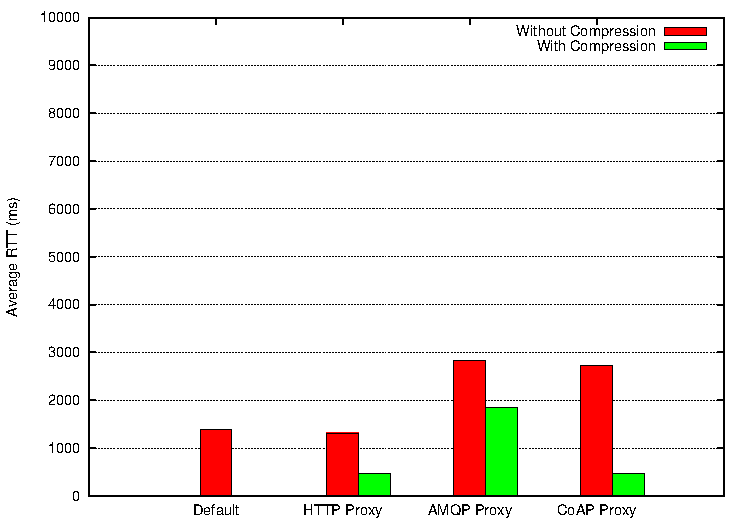
\includegraphics[width=0.5\textwidth]{../results/kongsberg/nffi/result.pdf}}
    \subfloat[REST]{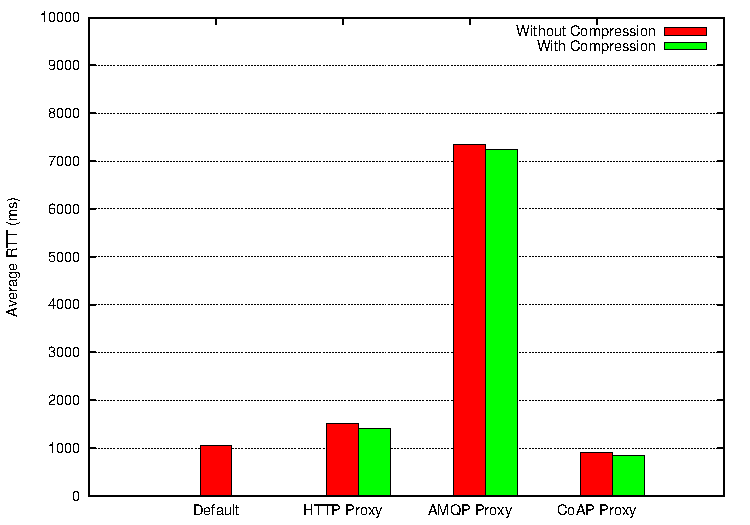
\includegraphics[width=0.5\textwidth]{../results/kongsberg/rest/result.pdf}}
    }{\caption{Tactical Broadband tests - Average RTT Time for the client application.}}
    \end{floatrow}
    \end{figure}
\end{landscape}

\section{Discussion}

Diskutere resultater. Ta opp at CoAP er veldig bra på små meldinger, men sliter
på store. Det er et kjent problem, og det er arbeid som gjøres for å spesifiere
mekansimer for gjøre dette anderledes.

\section{Summary}

In this section the results from the tests are presented. These results lead up
to the discussion and conclusion in the next chapter.

\begin{itemize}
\item AMQP has the worst performance in almost every test scenario.
\item Compression almost always yields an performance increase.
\item CoAP struggles with larger messages.
\item CoAP has the best performance with smaller messages in networks with low data rate.
\end{itemize}

\begin{table}[h]
\begin{tabular}{| l | l | l |}
\hline
  \textbf{Network} & \textbf{NFFI Web service recommendation} & \textbf{REST recommendation}\\ \hline
  \gls{satcom} & X & X \\ \hline
  \gls{los} & X & X\\ \hline
  WiFi 1 & X & X \\ \hline
  WiFi 2 & X & X \\ \hline
  \gls{cnr} & X & X \\ \hline
  Edge & X & X\\ \hline
\end{tabular}
\caption{Recommendations}
\label{table-evaluation-summary}
\end{table}
